%
% einleitung.tex -- Beispiel-File für die Einleitung
%
% (c) 2020 Prof Dr Andreas Müller, Hochschule Rapperswil
%
% !TEX root = ../../buch.tex
% !TEX encoding = UTF-8
%
\section{Geometrisch Physikalischer Beweis}
\label{basel:section:geombeweis}

Als erstes braucht man den \emph{Inversen Satz des Pythagoras},
bei diesem Satz geht es um den Kehrwert der Kathetenlängen.

\subsection{Herleitung}
\label{basel:subsection:invpythagoras}

Das Produkt der Kathetenlängen $ab$ ergibt die Flache eines Rechtecks,
das bekanntlich genau doppelt so gross wie das Dreieck ist.

\begin{figure}
\centering
\begin{tikzpicture}[>=latex, thick]
\coordinate (A) at (0,0);
\coordinate (B) at (4,0);
\coordinate (C) at (1.2,2.5);
\draw (A) -- node[below]{$c$} (B)
          -- node[right]{$a$} (C)
          -- node[left] {$b$} cycle;
% Höhe auf Hypotenuse
\pgfmathsetmacro{\hx}{(1.2*4 + 2.5*0)/(4)}
\coordinate (H) at (\hx, 0);
\draw[dashed] (C) -- node[right]{$h$} (H);
\draw ($(H)+(0.15,0)$) -- ++(0,0.15) -- ++(-0.15,0);
\end{tikzpicture}
\caption{Rechtwinkliges Dreieck mit Katheten $a$, $b$, Hypotenuse $c$ und
Höhe $h$ auf die Hypotenuse.
\label{basel:figure:dreieck}}
\end{figure}

Nun wird die Höhe des Dreieckes auf die Hypotenuse $c$ gefällt.
Auch hier wird die Fläche des Dreiecks verdoppelt: $ab = ch$.
Anschliessend wird die Summe der Quadrate der Kehrwerte der Kathetenlängen berechnet:
\[
    \frac{1}{a^2} + \frac{1}{b^2}
    =
    \frac{a^2 + b^2}{a^2 b^2}
    =
    \frac{c^2}{c^2 h^2}
    =
    \frac{1}{h^2}.
\]
Die Summe der Quadrate der Kehrwerte der Kathetenlängen ist also das Quadrat
des Kehrwertes der Höhe auf die Hypotenuse.

\subsection{Der Konstruktionsprozess}
\label{basel:subsection:konstruktion}

Man startet mit einem Kreis $k_0$ um einen Punkt $M_0$, der den Umfang $2$ hat.
Auf dem Kreis liegt ein Punkt $Z$, genau gegenüber liegt der Punkt $M_1$.
Der Durchmesser ergibt sich aus dem Umfang:
\[
    U = 2 = \pi d
    \qquad\Rightarrow\qquad
    d = \frac{2}{\pi} = |M_1 Z|.
\]

\begin{figure}
\centering
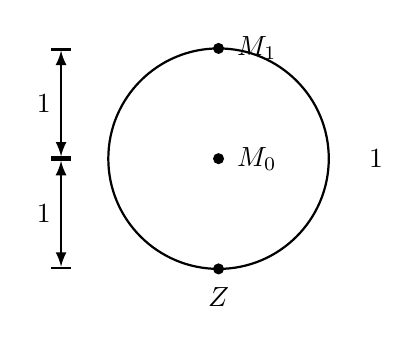
\begin{tikzpicture}[>=latex, thick]
\def\r{1.4}
\coordinate (M0) at (0,0);
\coordinate (M1) at (0,\r);
\coordinate (Z)  at (0,-\r);
\draw (M0) circle (\r);
\fill (M0) circle (2pt) node[right=3pt]{$M_0$};
\fill (M1) circle (2pt) node[right=3pt]{$M_1$};
\fill (Z)  circle (2pt) node[below=3pt]{$Z$};
\draw[|<->|] (-2.0,-\r) -- node[left]{$1$} (-2.0,0);
\draw[|<->|] (-2.0,0)   -- node[left]{$1$} (-2.0,\r);
\node at ( 2.0, 0) {$1$};
\node at (-2.0+0.6, 0) {};
\end{tikzpicture}
\caption{Ausgangskreis $k_0$ mit Umfang $2$, Mittelpunkt $M_0$,
oberem Punkt $M_1$ und unterem Punkt $Z$.
\label{basel:figure:k0}}
\end{figure}

Alle Intensitäten, die nachfolgend auf den Punkt $Z$ entfallen, werden berechnet;
daher wird $Z$ im Index nicht berücksichtigt.
Die Intensität von $M_1$ betragt
\[
    I(M_1)
    =
    \frac{1}{|M_1 Z|^2}
    =
    \frac{1}{d^2}
    =
    \frac{1}{\left(\dfrac{2}{\pi}\right)^2}
    =
    \frac{\pi^2}{4}.
\]
Es wird ein weiterer Kreis $k_1$ um den Punkt $M_1$ gezeichnet mit dem Radius $|M_1 Z|$.
Durch $M_1$ wird eine Senkrechte zu $ZM_1$ gezeichnet.
Dadurch erhält man die Punkte $P_{1,1}$ und $P_{1,2}$.
Daraus ergibt sich aus den Punkten $P_{1,1}$, $P_{1,2}$, $Z$ ein rechtwinkliges Dreieck
(Satz des Thales).
$M_1$ ist daher der Höhenfusspunkt in diesem Dreieck,
also wird die Intensität von $M_1$ auf die beiden Punkte $P_{1,1}$ und $P_{1,2}$ verteilt:
\[
    I(M_1) = \frac{\pi^2}{4} = I(P_{1,1}) + I(P_{1,2}).
\]

\begin{figure}
\centering
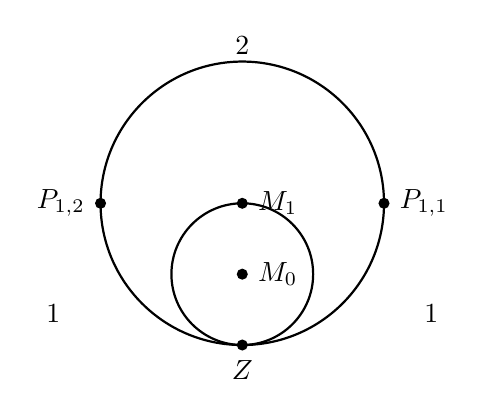
\begin{tikzpicture}[>=latex, thick]
\def\r{0.9}
\def\R{1.8}
\coordinate (M0)  at (0,0);
\coordinate (M1)  at (0,\r);
\coordinate (Z)   at (0,-\r);
\coordinate (P11) at (\R,\r);
\coordinate (P12) at (-\R,\r);
\draw (M0) circle (\r);
\draw (M1) circle (\R);
\fill (M0)  circle (2pt) node[right=2pt]{$M_0$};
\fill (M1)  circle (2pt) node[right=2pt]{$M_1$};
\fill (Z)   circle (2pt) node[below=2pt]{$Z$};
\fill (P11) circle (2pt) node[right=2pt]{$P_{1,1}$};
\fill (P12) circle (2pt) node[left=2pt] {$P_{1,2}$};
\node at (0,  2.9) {$2$};
\node at ( 2.4, -0.5) {$1$};
\node at (-2.4, -0.5) {$1$};
\end{tikzpicture}
\caption{Erster Konstruktionsschritt: Kreis $k_1$ um $M_1$ mit den Punkten
$P_{1,1}$ und $P_{1,2}$.
Die Bogenlängen betragen: $P_{1,1}P_{1,2}=2$, $P_{1,2}Z=1$, $ZP_{1,1}=1$.
\label{basel:figure:k1}}
\end{figure}

Um $M_2$ wird ein weiterer Kreis $k_2$ mit dem Radius $|M_2 Z|$ gezeichnet.
Die Gerade $M_2 P_{1,1}$ erzeugt auf dem Kreis $k_2$ die Punkte $P_{2,1}$ und $P_{2,3}$,
die Gerade $M_2 P_{1,2}$ die Punkte $P_{2,2}$ und $P_{2,4}$.
Das Dreieck $P_{2,1} P_{2,3} Z$ steht rechtwinklig mit dem rechten Winkel bei $Z$
(Satz des Thales).
$P_{1,1}$ ist somit der Höhenfusspunkt in diesem Dreieck.
Somit kann die Intensität von $P_{1,1}$ auf die beiden Punkte $P_{2,1}$ und $P_{2,3}$
verteilt werden:
\[
    I(P_{1,1}) = I(P_{2,1}) + I(P_{2,3}).
\]
Analog wird das Dreieck $P_{2,2} P_{2,4} Z$ rechtwinklig mit dem rechten Winkel bei $Z$
(Satz des Thales).
$P_{1,2}$ ist der Höhenfusspunkt in diesem Dreieck.
Deshalb kann die Intensität von $P_{1,2}$ auf die beiden Punkte $P_{2,2}$ und $P_{2,4}$
verteilt werden.
Also gilt insgesamt:
\[
    I(P_{1,1}) + I(P_{1,2})
    =
    I(P_{2,1}) + I(P_{2,3}) + I(P_{2,2}) + I(P_{2,4})
    =
    \frac{\pi^2}{4}.
\]
%ACHTUNG ACHTUNG ACHTUNG FALSCH FALSCH FALSCH
%ACHTUNG ACHTUNG ACHTUNG FALSCH FALSCH FALSCH
%ACHTUNG ACHTUNG ACHTUNG FALSCH FALSCH FALSCH
%ACHTUNG ACHTUNG ACHTUNG FALSCH FALSCH FALSCH
\begin{figure}
\centering
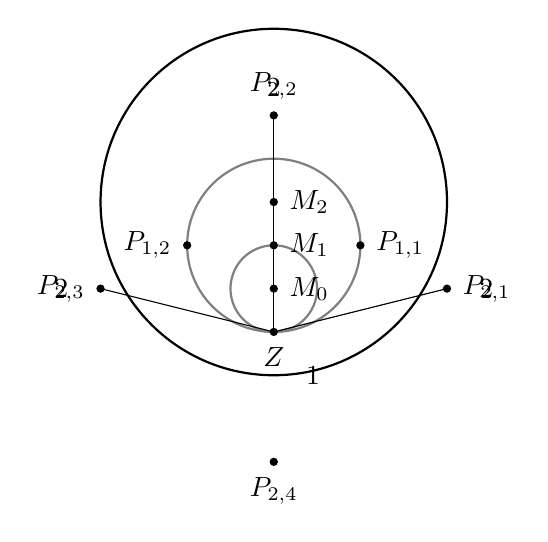
\begin{tikzpicture}[>=latex, thick]
\def\ra{0.55}
\def\rb{1.10}
\def\rc{2.20}
\coordinate (M0)  at (0,0);
\coordinate (M1)  at (0,\ra);
\coordinate (M2)  at (0,\rb);
\coordinate (Z)   at (0,-\ra);
\coordinate (P11) at (\rb,\ra);
\coordinate (P12) at (-\rb,\ra);
\coordinate (P21) at (\rc, 0);
\coordinate (P22) at (0, \rc);
\coordinate (P23) at (-\rc, 0);
\coordinate (P24) at (0, -\rc);
\draw[gray] (M0) circle (\ra);
\draw[gray] (M1) circle (\rb);
\draw       (M2) circle (\rc);
\draw[thin] (Z) -- (P21);
\draw[thin] (Z) -- (P22);
\draw[thin] (Z) -- (P23);
\fill (M0)  circle (1.5pt) node[right=2pt]{$M_0$};
\fill (M1)  circle (1.5pt) node[right=2pt]{$M_1$};
\fill (M2)  circle (1.5pt) node[right=2pt]{$M_2$};
\fill (Z)   circle (1.5pt) node[below=2pt]{$Z$};
\fill (P11) circle (1.5pt) node[right=2pt]{$P_{1,1}$};
\fill (P12) circle (1.5pt) node[left=2pt] {$P_{1,2}$};
\fill (P21) circle (1.5pt) node[right=2pt]{$P_{2,1}$};
\fill (P22) circle (1.5pt) node[above=2pt]{$P_{2,2}$};
\fill (P23) circle (1.5pt) node[left=2pt] {$P_{2,3}$};
\fill (P24) circle (1.5pt) node[below=2pt]{$P_{2,4}$};
\node at (0,   \rc+0.35) {$2$};
\node at (\rc+0.5, 0)    {$2$};
\node at (-\rc-0.5, 0)   {$2$};
\node at (0.5, -\rc*0.5) {$1$};
\end{tikzpicture}
\caption{Zweiter Konstruktionsschritt: Kreis $k_2$ mit den Punkten
$P_{2,1}$, $P_{2,2}$, $P_{2,3}$, $P_{2,4}$.
\label{basel:figure:k2}}
\end{figure}
%ACHTUNG ACHTUNG ACHTUNG FALSCH FALSCH FALSCH
%ACHTUNG ACHTUNG ACHTUNG FALSCH FALSCH FALSCH
%ACHTUNG ACHTUNG ACHTUNG FALSCH FALSCH FALSCH
%ACHTUNG ACHTUNG ACHTUNG FALSCH FALSCH FALSCH
Der Kreis $k_2$ ist doppelt so gross wie $k_1$,
dementsprechend hat er also den Umfang $8$.
Die Bogen zwischen den Punkten haben folgende Längen:
\[
    Z P_{2,1} = 1,\quad
    P_{2,1} P_{2,2} = 2,\quad
    P_{2,2} P_{2,3} = 2,\quad
    P_{2,3} P_{2,4} = 2,\quad
    P_{2,4} Z = 1.
\]

Um $M_3$ wird ein Kreis $k_3$ mit einem Radius von $|M_3 Z|$ gezeichnet.
Hier als Beispiel: das Dreieck $P_{3,2} P_{3,6} Z$ ist rechtwinklig mit dem rechten Winkel
bei $Z$ (Satz des Thales).
$P_{2,2}$ ist also der Höhenfusspunkt in diesem Dreieck,
also wird die Intensität von $P_{2,2}$ auf die beiden Punkte $P_{3,2}$ und $P_{3,6}$
verteilt werden.
Dies gilt für jeden Punkt, welcher auf $k_2$ liegt.
Es können also alle Intensitäten aller Punkte von $k_2$ auf die entsprechenden Punkte
von $k_3$ verteilt werden.
%ACHTUNG ACHTUNG ACHTUNG FALSCH FALSCH FALSCH
%ACHTUNG ACHTUNG ACHTUNG FALSCH FALSCH FALSCH
%ACHTUNG ACHTUNG ACHTUNG FALSCH FALSCH FALSCH
%ACHTUNG ACHTUNG ACHTUNG FALSCH FALSCH FALSCH
\begin{figure}
\centering
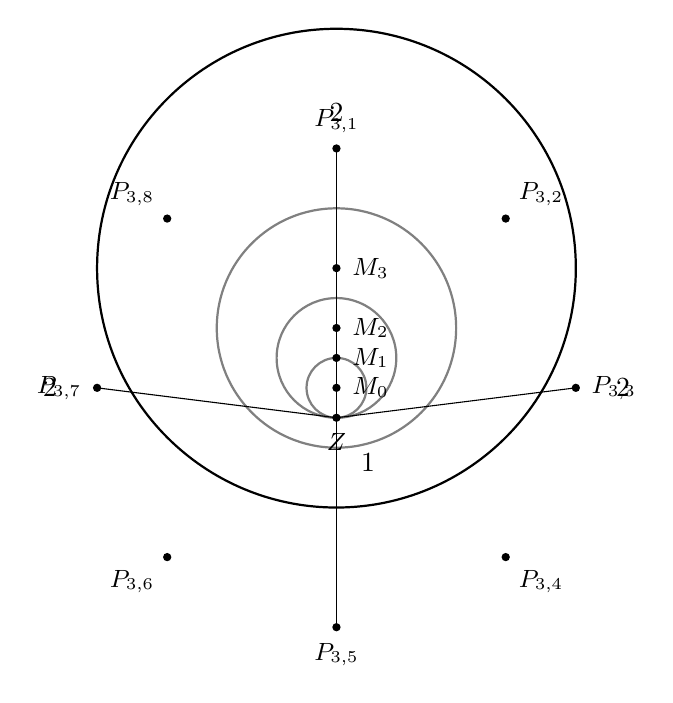
\begin{tikzpicture}[>=latex, thick]
\def\ra{0.38}
\def\rb{0.76}
\def\rc{1.52}
\def\rd{3.04}
\coordinate (M0) at (0,0);
\coordinate (M1) at (0,\ra);
\coordinate (M2) at (0,\rb);
\coordinate (M3) at (0,\rc);
\coordinate (Z)  at (0,-\ra);
% 8 Punkte auf k3 gleichmässig verteilt, Start oben
\coordinate (Pa) at (90:\rd);
\coordinate (Pb) at (45:\rd);
\coordinate (Pc) at (0:\rd);
\coordinate (Pd) at (-45:\rd);
\coordinate (Pe) at (-90:\rd);
\coordinate (Pf) at (-135:\rd);
\coordinate (Pg) at (180:\rd);
\coordinate (Ph) at (135:\rd);
\draw[gray] (M0) circle (\ra);
\draw[gray] (M1) circle (\rb);
\draw[gray] (M2) circle (\rc);
\draw       (M3) circle (\rd);
\draw[thin] (Z) -- (Pa);
\draw[thin] (Z) -- (Pc);
\draw[thin] (Z) -- (Pe);
\draw[thin] (Z) -- (Pg);
\fill (M0) circle (1.5pt) node[right=2pt]{\small$M_0$};
\fill (M1) circle (1.5pt) node[right=2pt]{\small$M_1$};
\fill (M2) circle (1.5pt) node[right=2pt]{\small$M_2$};
\fill (M3) circle (1.5pt) node[right=2pt]{\small$M_3$};
\fill (Z)  circle (1.5pt) node[below=2pt]{\small$Z$};
\fill (Pa) circle (1.5pt) node[above=2pt]{\small$P_{3,1}$};
\fill (Pb) circle (1.5pt) node[above right=1pt]{\small$P_{3,2}$};
\fill (Pc) circle (1.5pt) node[right=2pt]{\small$P_{3,3}$};
\fill (Pd) circle (1.5pt) node[below right=1pt]{\small$P_{3,4}$};
\fill (Pe) circle (1.5pt) node[below=2pt]{\small$P_{3,5}$};
\fill (Pf) circle (1.5pt) node[below left=1pt]{\small$P_{3,6}$};
\fill (Pg) circle (1.5pt) node[left=2pt]{\small$P_{3,7}$};
\fill (Ph) circle (1.5pt) node[above left=1pt]{\small$P_{3,8}$};
\node at (0,    \rd+0.45) {$2$};
\node at (\rd+0.6,  0)    {$2$};
\node at (-\rd-0.6, 0)    {$2$};
\node at (0.4, -\ra*2.5)  {$1$};
\end{tikzpicture}
\caption{Dritter Konstruktionsschritt: Kreis $k_3$ mit acht äquidistanten Punkten.
\label{basel:figure:k3}}
\end{figure}
%ACHTUNG ACHTUNG ACHTUNG FALSCH FALSCH FALSCH
%ACHTUNG ACHTUNG ACHTUNG FALSCH FALSCH FALSCH
%ACHTUNG ACHTUNG ACHTUNG FALSCH FALSCH FALSCH
%ACHTUNG ACHTUNG ACHTUNG FALSCH FALSCH FALSCH
Dadurch gibt es zwei Konstanten bei diesem schrittweisen Konstruktionsprozess.
Die Summe aller Intensitäten aller Punkte auf einem Kreis bleibt $\dfrac{\pi^2}{4}$.
Entsprechend der Vorbereitung liegen die Punkte auf einem Kreis äquidistant
(gleiche Abstände aufweisend) und die Bögen haben konstant die Länge $2$.

\subsection{Der Grenzübergang}
\label{basel:subsection:grenzuebergang}

Im Grenzübergang erhält man einen unendlich grossen Kreis durch $Z$,
besser gesagt eine Gerade durch $Z$.
Wegen den konstanten Bogenlängen $1, 2, 2, \ldots$ liegen die Punkte der Geraden
im Abstand $1, 3, 5, 7, \ldots$ zu beiden Seiten von $Z$.

Die Summe aller Intensitäten beträgt immer noch $\dfrac{\pi^2}{4}$:
\[
    \bigl(I(P_1) + I(P_2) + I(P_3) + I(P_4) + \cdots\bigr)
    +
    \bigl(I(P_{-1}) + I(P_{-2}) + I(P_{-3}) + I(P_{-4}) + \cdots\bigr)
    =
    \frac{\pi^2}{4}.
\]
Wegen der Symmetrie gilt jedoch:
\[
    I(P_1) + I(P_2) + I(P_3) + I(P_4) + \cdots
    =
    \frac{\pi^2}{8}.
\]
Die Intensitäten können nun explizit bestimmt werden.
Da die Punkte im Abstand $1, 3, 5, 7, \ldots$ von $Z$ liegen, ergibt sich
\[
    \frac{1}{1^2} + \frac{1}{3^2} + \frac{1}{5^2} + \frac{1}{7^2}
    + \frac{1}{9^2} + \cdots
    =
    \frac{\pi^2}{8}
    =: S_u.
\]
Das Ziel der Betrachtung ist $S_u = \dfrac{\pi^2}{8}$.
Nun setzt man die vollständige Reihe zusammen:
\begin{align*}
    S
    &=
    \frac{1}{1^2} + \frac{1}{2^2} + \frac{1}{3^2} + \frac{1}{4^2}
    + \frac{1}{5^2} + \frac{1}{6^2} + \frac{1}{7^2} + \frac{1}{8^2}
    + \cdots
    =
    S_u + S_g,
    \\
    S_g
    &=
    \frac{1}{2^2} + \frac{1}{4^2} + \frac{1}{6^2} + \frac{1}{8^2} + \cdots
    =
    \frac{1}{2^2}
    \left(
        \frac{1}{1^2} + \frac{1}{2^2} + \frac{1}{3^2} + \frac{1}{4^2} + \cdots
    \right)
    =
    \frac{1}{4} S.
\end{align*}
Also gilt
\[
    S
    =
    S_u + S_g
    =
    \frac{\pi^2}{8} + \frac{1}{4} S
    \qquad\Rightarrow\qquad
    \frac{3}{4} S = \frac{\pi^2}{8}
    \qquad\Rightarrow\qquad
    S = \frac{\pi^2}{8} \cdot \frac{4}{3},
\]
und damit
\begin{equation}
    S
    =
    \frac{\pi^2}{6}.
    \label{basel:equation:resultatgeom}
\end{equation}
